\documentclass{beamer}
\usepackage{listings}
\usetheme{Copenhagen}
\usecolortheme{beaver}
\setbeamertemplate{navigation symbols}{}
\setbeamertemplate{footline}{\parbox[t][12pt][c]{12pt}{~\scriptsize\insertframenumber}}
% \usepackage{beamerthemesplit} // Activate for custom appearance

%%%%%%%%%%%%
% MVS: Language definitions
%
\renewcommand{\ttdefault}{pcr}
\lstset{
  basicstyle=\small\ttfamily,
  breaklines=true
}
\lstdefinelanguage{cvl}{
  morekeywords={generalize,to, with, other, at, zoom, levels, weigh, by, subject, and, create, constraint, as, not, exists, resolve, if, delete, select, from, where, in, order, over, setup, teardown,force,min,level,for,allornothing,join,on,setup,group,having,index,temporary,table,drop,partition,merge,partitions},
  sensitive=false,
  morecomment=[l]{//},
  morecomment=[s]{/*}{*/},
  morestring=[b]",
}
\lstset{
  language=cvl
}


\title{Declarative Cartography}
\subtitle{In-Database Map Generalization of Spatial Datasets}
\author{\underline{Pimin Konstantin Kefaloukos}, Marcos Vaz Salles, \\Martin Zachariasen\\ \small{\emph{Computer Science Department (DIKU)}, \textbf{University of Copenhagen}}}
\date{\today}

\begin{document}

\frame{\titlepage}

\frame
{
  \frametitle{Motivation}
  \begin{itemize}
  \item \textbf{Imagine}: you're a \emph{journalist} and want to tell a story about restaurants in Z\"{u}rich \emph{using a map}.
  \item \textbf{Database}: You have a \emph{database} of restaurants (unique ID, location, star rating, name etc.)
  \item Simply showing all the records creates a mess (see picture)
  \item Generalization of overlays is an important problem, with increasing use cases
  \end{itemize}
  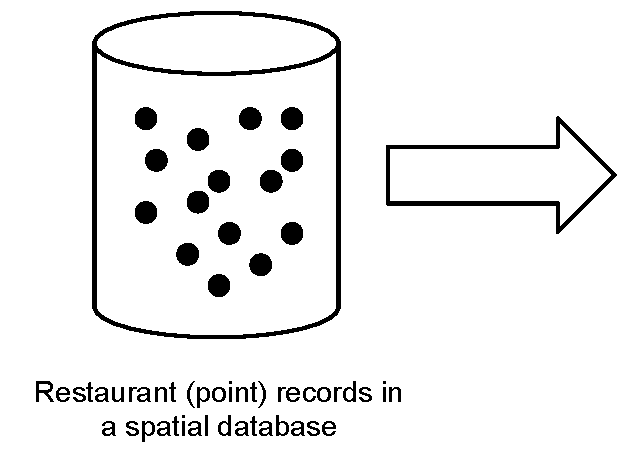
\includegraphics[scale=0.5]{figs/spatial-database-with-points.pdf} 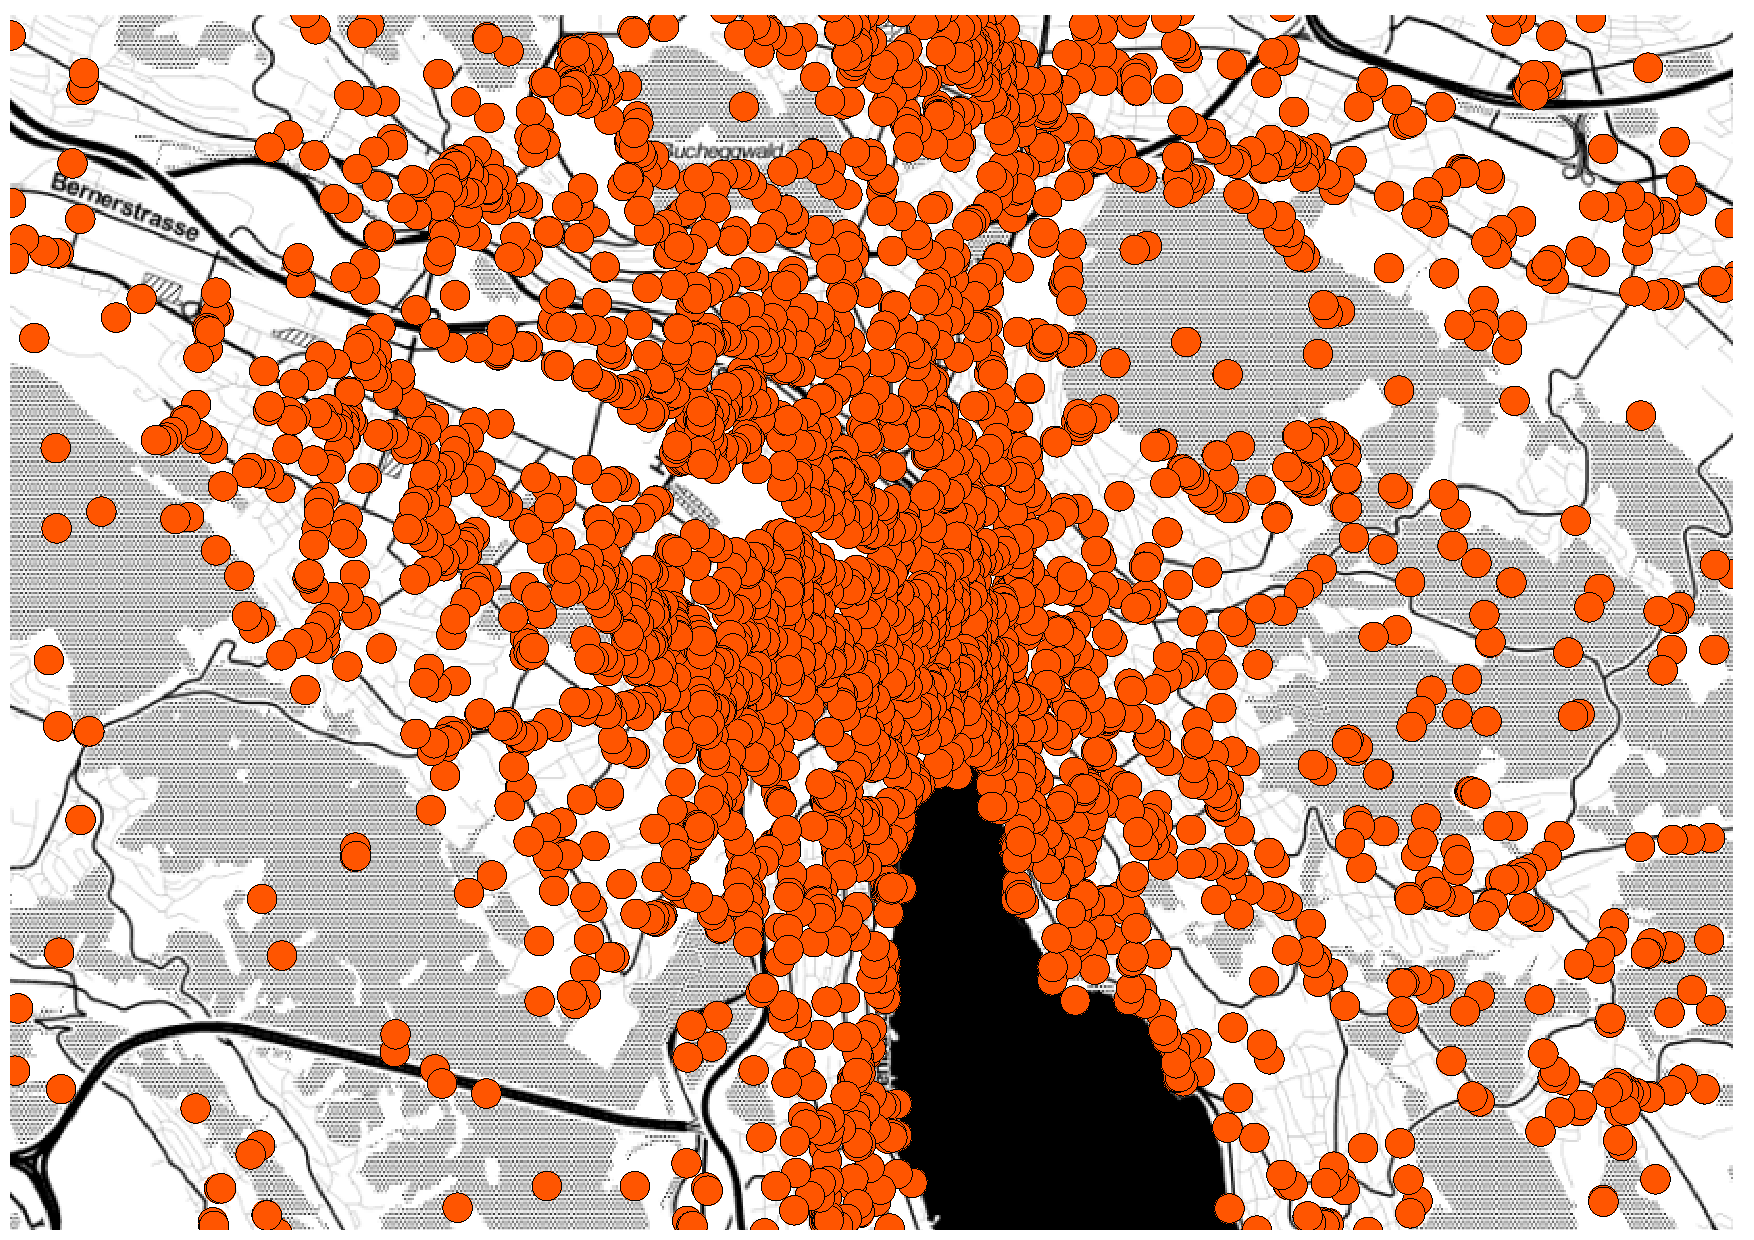
\includegraphics[scale=0.18]{figs/zurich-unfiltered.pdf}
}

% Setting stage
\frame[t]
{
  \frametitle{What a good (thematic) map might look like}
\begin{columns}[t]
	\begin{column}[l]{6cm}
		\begin{itemize}[<+->]
			\item Records should appear \emph{gradually} when zooming in, i.e. \emph{constant information~density}
			\item ``Important'' records should get priority
			\item Visible records should \emph{remain visible} when zooming in
			\item There should be some way of controlling \emph{layout}
		\end{itemize}
	\end{column}
	\begin{column}[l]{6cm}
    \begin{figure}
    	\includegraphics<1>[scale=0.18]{figs/zoom12.pdf}
        \includegraphics<2>[scale=0.18]{figs/zoom13.pdf}
        \includegraphics<3>[scale=0.18]{figs/zoom14.pdf}
        \includegraphics<4>[scale=0.18]{figs/zoom15.pdf}
        \includegraphics<5>[scale=0.18]{figs/zoom16.pdf}
    \end{figure}                            
\end{column}
\end{columns}
}

% Setting stage
\frame[t]
{
  \frametitle{Spatial databases}
	\begin{itemize}[<+->]
		\item Spatial data is often stored in a \emph{spatial database}
		\item They have powerful capabilities
		\item \emph{joins}, \emph{sorting}, \emph{spatial indexing} and \emph{spatial functions}
	\end{itemize}
	\begin{center}
	\begin{figure}
    		\includegraphics<1>[scale=0.3]{figs/cvl-powerful-database.pdf}
    		\includegraphics<2>[scale=0.3]{figs/cvl-powerful-database.pdf}
		\includegraphics<3>[scale=0.3]{figs/cvl-powerful-database-2.pdf}
	\end{figure}       
	\end{center}                     
}

\frame[t]
{
  \frametitle{External software}
	\begin{itemize}[<+->]
		\item The ``normal'' way is to pull the data out of the \emph{database}
		\item Process the data in external software, i.e. implement generalization algorithms
		\item Put the data back into the database when done
		\item \emph{Several drawbacks}: re-inventing the wheel, memory and bandwidth limits, serialization costs, deployment
	\end{itemize}
	\begin{center}
	\begin{figure}
    		\includegraphics<1>[scale=0.3]{figs/cvl-external-software-out.pdf}
    		\includegraphics<2>[scale=0.3]{figs/cvl-external-software-proc.pdf}
		\includegraphics<3>[scale=0.3]{figs/cvl-external-software-in.pdf}
		\includegraphics<4>[scale=0.3]{figs/cvl-external-software-rest.pdf}
	\end{figure}       
	\end{center}                     
}

\frame[t]
{
  \frametitle{Code-to-data}
	\begin{itemize}[<+->]
		\item Instead, state intensions in a high-level generalization language
		\item Transform statement into a program that the database can execute
		\item ``Code-to-data'' instead of ``data-to-code-and-back''
	\end{itemize}
	\begin{center}
	\begin{figure}
    		\includegraphics<1>[scale=0.3]{figs/cvl-state-intension.pdf}
    		\includegraphics<2>[scale=0.3]{figs/cvl-compile-statement.pdf}
		\includegraphics<3>[scale=0.3]{figs/cvl-code-to-data.pdf}
	\end{figure}       
	\end{center}                     
}




\end{document}